\chapter{Versuch 1}
\label{chap:VERSUCH_1}


\section{Fragestellung, Messprinzip, Aufbau, Messmittel}
\label{chap:VERSUCH_1_FRAGESTELLUNG}

\subsection*{Fragesetellung}

Ziel war es eine Aufnahme von einen Grauwertkeil zu erstellen, damit dieser auf seine Bildfehler untersucht und später korrigiert werden kann.
Für einen besseren Vergleich soll zudem der Mittelwert und die Standardabweichung zu jeden der fünf Grauwerte ermittelt werden, damit diese mit den entsprechenden Werten des korrigierten Bilds verglichen werden können.

\subsection*{Messprinzip}
Der Grauwertkeiler stellt einen stufenweise Grauwertverlauf dar, 

\subsection*{Aufbau}

\subsection*{Messmittel}
\begin{itemize}
\item Webcame (Asus USB2.0 UVC HD Webcam)
\item Grauwertkeil
\item Metermaß
\end{itemize}

\section{Messwerte}
\label{chap:VERSUCH_1_MESSWERTE}

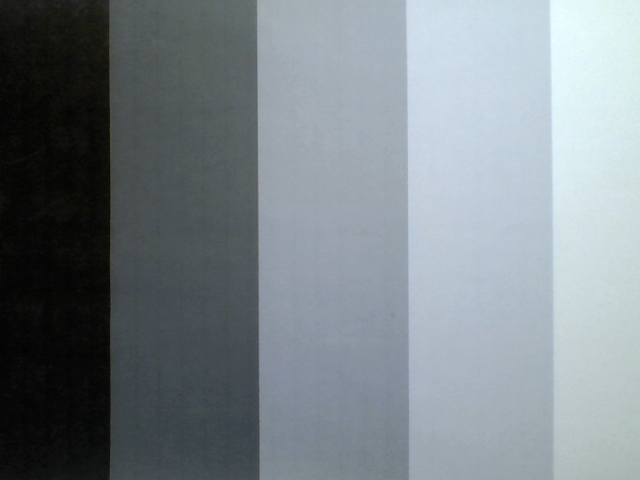
\includegraphics[scale=0.7]{media/grauwertkeil/grauwertkeil.png}
\captionof{figure}{Fig: Grauwertkeil, unbearbeitet}
\label{Fig:Grawertkeil}


\section{Auswertung}
\label{chap:VERSUCH_1_AUSWERTUNG}

Zur Auswertung des Grauwertkeil-Bildes wird das Bild zunächst in fünf Abschnitte unterteilt. Jeder Abschnitt soll eine der Graustufen enthalten und dabei so viele Pixel wie möglich umfassen, so dass der Abschnitt keine Pixel der anderen Graustufen enthält.

Für jeden Abschnitt wird dann ein Mittelwert bestimmt, der idealerweise der wahre Grauwert des Abschnitts wäre.
Zudem wird die Standardabweichung von jeder Stufe ermittelt, wobei es wichtig ist die Standardabweichung über alle Werte der jeweiligen Stufe zu ermitteln, und nicht die des Mittelwerts.

\subsection*{Mittelwerte und Standardabweichung des Grauwertkeilers}

\begin{tabular}{|c|c|c|}
\hline 
Graustufe & Mittelwert & Standardabweichung \\ 
\hline 
0 (schwarz) & 10.37 & 5.32 \\ 
\hline 
1 (dunkelgrau) & 79.53 & 9.78 \\ 
\hline 
2 (mittelgrau) & 155.67 & 14.55 \\ 
\hline 
3 (hellgrau) & 193.70 & 17.36 \\ 
\hline 
4 (weiß) & 215.66 & 18.65 \\ 
\hline 
\end{tabular} 
\captionof{table}{Tab:Grauwert1}

\section{Interpretation}
\label{chap:VERSUCH_1_INTERPRETATION}

Die Mittelwerte zeigen, dass wie erwartet die dunklere Graustufen auch niedrigere Werte haben. Wobei es interessant ist das die dunkelste Stufe dennoch nicht bei 0 liegt.

Die Standardabweichung wird größer je heller die werte sind